% Options for packages loaded elsewhere
\PassOptionsToPackage{unicode}{hyperref}
\PassOptionsToPackage{hyphens}{url}
\PassOptionsToPackage{dvipsnames,svgnames,x11names}{xcolor}
%
\documentclass[
  ignorenonframetext,
]{beamer}
\usepackage{pgfpages}
\setbeamertemplate{caption}[numbered]
\setbeamertemplate{caption label separator}{: }
\setbeamercolor{caption name}{fg=normal text.fg}
\beamertemplatenavigationsymbolsempty
% Prevent slide breaks in the middle of a paragraph
\widowpenalties 1 10000
\raggedbottom
\setbeamertemplate{part page}{
  \centering
  \begin{beamercolorbox}[sep=16pt,center]{part title}
    \usebeamerfont{part title}\insertpart\par
  \end{beamercolorbox}
}
\setbeamertemplate{section page}{
  \centering
  \begin{beamercolorbox}[sep=12pt,center]{part title}
    \usebeamerfont{section title}\insertsection\par
  \end{beamercolorbox}
}
\setbeamertemplate{subsection page}{
  \centering
  \begin{beamercolorbox}[sep=8pt,center]{part title}
    \usebeamerfont{subsection title}\insertsubsection\par
  \end{beamercolorbox}
}
\AtBeginPart{
  \frame{\partpage}
}
\AtBeginSection{
  \ifbibliography
  \else
    \frame{\sectionpage}
  \fi
}
\AtBeginSubsection{
  \frame{\subsectionpage}
}
\usepackage{amsmath,amssymb}
\usepackage{iftex}
\ifPDFTeX
  \usepackage[T1]{fontenc}
  \usepackage[utf8]{inputenc}
  \usepackage{textcomp} % provide euro and other symbols
\else % if luatex or xetex
  \usepackage{unicode-math} % this also loads fontspec
  \defaultfontfeatures{Scale=MatchLowercase}
  \defaultfontfeatures[\rmfamily]{Ligatures=TeX,Scale=1}
\fi
\usepackage{lmodern}
\ifPDFTeX\else
  % xetex/luatex font selection
\fi
% Use upquote if available, for straight quotes in verbatim environments
\IfFileExists{upquote.sty}{\usepackage{upquote}}{}
\IfFileExists{microtype.sty}{% use microtype if available
  \usepackage[]{microtype}
  \UseMicrotypeSet[protrusion]{basicmath} % disable protrusion for tt fonts
}{}
\makeatletter
\@ifundefined{KOMAClassName}{% if non-KOMA class
  \IfFileExists{parskip.sty}{%
    \usepackage{parskip}
  }{% else
    \setlength{\parindent}{0pt}
    \setlength{\parskip}{6pt plus 2pt minus 1pt}}
}{% if KOMA class
  \KOMAoptions{parskip=half}}
\makeatother
\usepackage{xcolor}
\newif\ifbibliography
\usepackage{graphicx}
\makeatletter
\def\maxwidth{\ifdim\Gin@nat@width>\linewidth\linewidth\else\Gin@nat@width\fi}
\def\maxheight{\ifdim\Gin@nat@height>\textheight\textheight\else\Gin@nat@height\fi}
\makeatother
% Scale images if necessary, so that they will not overflow the page
% margins by default, and it is still possible to overwrite the defaults
% using explicit options in \includegraphics[width, height, ...]{}
\setkeys{Gin}{width=\maxwidth,height=\maxheight,keepaspectratio}
% Set default figure placement to htbp
\makeatletter
\def\fps@figure{htbp}
\makeatother
\setlength{\emergencystretch}{3em} % prevent overfull lines
\providecommand{\tightlist}{%
  \setlength{\itemsep}{0pt}\setlength{\parskip}{0pt}}
\setcounter{secnumdepth}{-\maxdimen} % remove section numbering
% mystyle3.tex
\usepackage{graphicx}
\titlegraphic{
    
\includegraphics[height=1.5cm]{UniUrb-logo.png}\hfill
    
\includegraphics[height=1.5cm]{bremen_logo.png}
}

 \definecolor{myblue}{HTML}{005997}
  \setbeamercolor{frametitle}{fg=myblue}
    \setbeamercolor{framesubtitle}{fg=myblue}
    \setbeamercolor{frametitle right}{fg=myblue}
  \setbeamercolor{titlelike}{fg=myblue}
    \setbeamercolor{title}{fg=myblue}
      \setbeamercolor{subtitle}{fg=myblue}
    \setbeamercolor{part title}{fg=myblue}
    \setbeamercolor{section title}{fg=myblue}
    \setbeamercolor{subsection title}{fg=myblue}
  \setbeamercolor{section name}{fg=myblue}
  \setbeamercolor{subsection name}{fg=myblue}
  \setbeamercolor{part name}{fg=myblue}
  \setbeamercolor{title in head/foot}{fg=myblue}
  \setbeamercolor{subtitle in head/foot}{fg=myblue}
  \setbeamercolor{block title}{fg=myblue}
  
  \setbeamercolor{bullet}{fg=myblue}
  \setbeamercolor{section in toc}{fg=myblue}
  \setbeamercolor{subsection in toc}{fg=myblue}
  \setbeamercolor{section in head/foot}{fg=myblue}
  \setbeamercolor{subsection in head/foot}{fg=myblue}
  
  
  \setbeamercolor{itemize item}{fg = myblue}
  \setbeamercolor{itemize subitem}{fg = myblue}
  \setbeamercolor{itemize subsubitem}{fg = myblue}
  \setbeamercolor{enumerate item}{fg = myblue}
  \setbeamercolor{enumerate subitem}{fg = myblue}
  \setbeamercolor{enumerate subsubitem}{fg = myblue}
\usepackage{etoolbox}
\AtBeginEnvironment{thebibliography}{\scriptsize}
\ifLuaTeX
  \usepackage{selnolig}  % disable illegal ligatures
\fi
\usepackage[round]{natbib}
\bibliographystyle{plainnat}
\usepackage{bookmark}
\IfFileExists{xurl.sty}{\usepackage{xurl}}{} % add URL line breaks if available
\urlstyle{same}
\hypersetup{
  pdftitle={Tracking the Digital Divide: Factor Analysis and Time Trends in Italian Firms},
  pdfauthor={Luis Carlos Castillo},
  colorlinks=true,
  linkcolor={myblue},
  filecolor={Maroon},
  citecolor={Blue},
  urlcolor={Blue},
  pdfcreator={LaTeX via pandoc}}

\title{Tracking the Digital Divide: Factor Analysis and Time Trends in
Italian Firms}
\author{Luis Carlos Castillo}
\date{30 June 2024}
\institute{Binational Doctorate\\
University of Urbino and Universty of Bremen\\
Ph.D.~Program in Global Studies\\
Supervisor: Prof.~Francesco Vidoli\\
Co-Supervisor: Prof.~Dr.~Christian Cordes}

\begin{document}
\frame{\titlepage}

\begin{frame}{Cumulative Dissertation}
\phantomsection\label{cumulative-dissertation}
\begin{center}
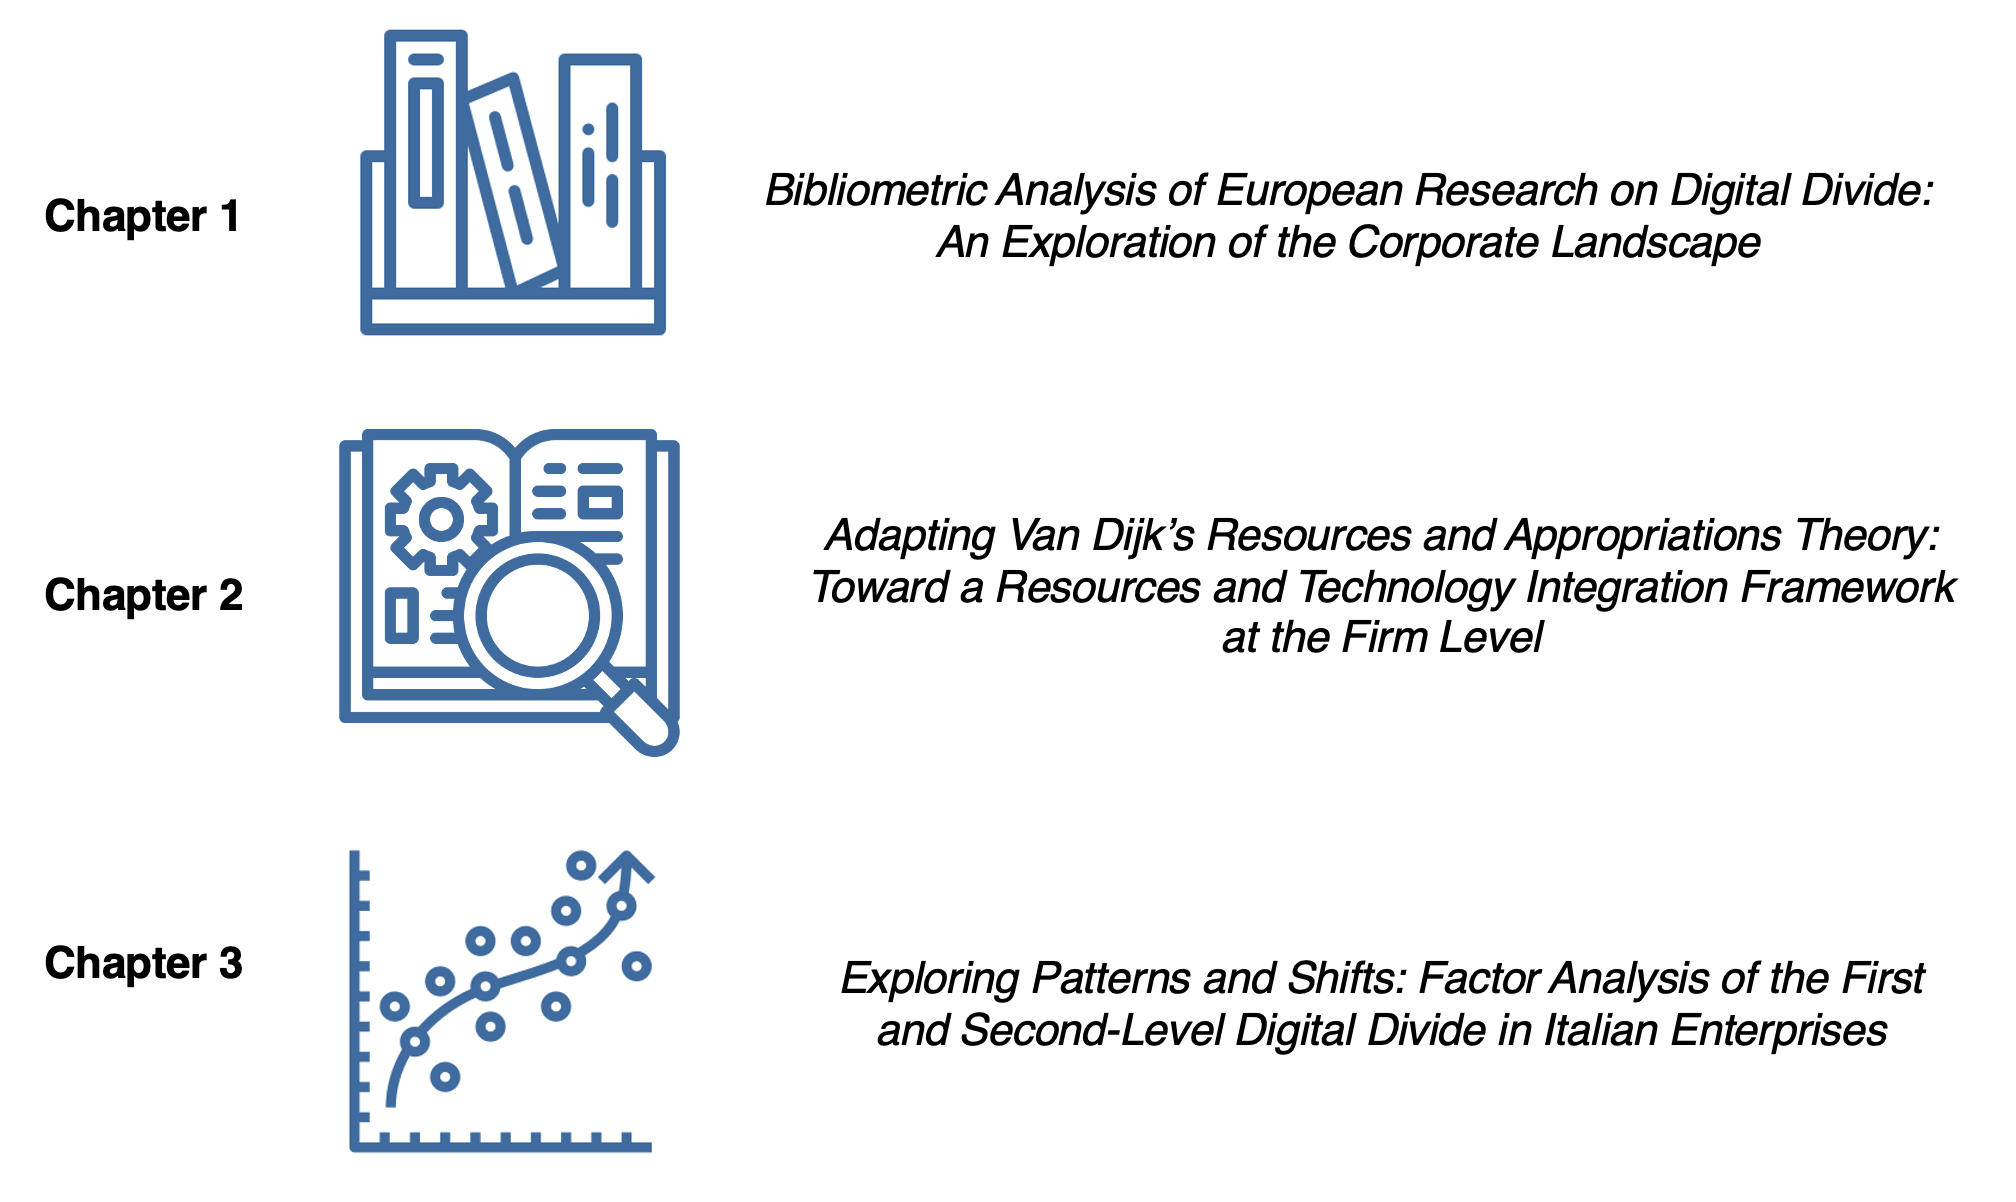
\includegraphics[width=1\textwidth, height=0.75\textheight]{structure_thesis.png}
\end{center}
\end{frame}

\begin{frame}{1. Introduction}
\phantomsection\label{introduction}
\begin{itemize}
\item
  DT play a pivotal role in reshaping business models
  \citep{trischler2023} , driving innovation \citep{ciarli2021}, and
  fostering competitive advantages \citep{jeganjosephjerome2024}.
\item
  The unequal adoption of DT has led to significant challenge: the
  digital divide.
\item
  The digital divide at the firm level is a multifaceted gap
  characterized not only by disparities in access, skills and usage of
  DT, but also the derived benefits from different types of use.
\item
  While the digital divide is a global issue, its impact on enterprises,
  especially in Italy, presents unique challenges and opportunities.
\end{itemize}
\end{frame}

\begin{frame}{2. Objectives}
\phantomsection\label{objectives}
\begin{itemize}
\item
  Develop composite indices to track trends in the first and
  second-level digital divide.
\item
  Analyze variations in the first and second-level digital divide across
  firm sizes, sectors, and regions in Italy.
\item
  Evaluate the alignment of resources and technology integration theory
  with observed data.
\item
  Propose targeted policy interventions based on research findings.
\end{itemize}
\end{frame}

\begin{frame}{3.1. Research Questions}
\phantomsection\label{research-questions}
\begin{itemize}
\item
  How does the Resources and Technology Integration theory reflect
  observed patterns in DT adoption across different Italian enterprises?
\item
  What are the evolving patterns and shifts in access, skills, and usage
  among Italian enterprises, and how do these dynamics reflect the
  disparities between the three indices across different firm sizes,
  sectors, and regions over a six-year period?
\item
  According to the findings, what policy interventions can be
  recommended to help Italian enterprises more effectively bridge the
  digital divide?
\end{itemize}
\end{frame}

\begin{frame}{5. Data}
\phantomsection\label{data}
\begin{itemize}
\item
  The dataset was derived from the ICT Usage in Enterprises Survey
  conducted annually between 2014 and 2019 by ISTAT.
\item
  In total, 29 variables were used to extract three factors that
  represent the theoretical constructs.

  \begin{itemize}
  \tightlist
  \item
    Access index: 6 variables
  \item
    Skills index: 9 variables
  \item
    Usage index: 11 variables
  \item
    \textbf{Control variable:} Firm size with three categories (small,
    medium, large)
  \end{itemize}
\item
  Considerations and Limitations.

  \begin{itemize}
  \tightlist
  \item
    Independence of Annual Data
  \end{itemize}
\item
  Data treatments, codes, and summary statistics, are available on my
  \href{https://github.com/luchocastillo84/Factor_Analysis_Digital_Divide/tree/main}{GitHub
  repository} for replicability and further analysis.
\end{itemize}
\end{frame}

\begin{frame}{6 Methodology}
\phantomsection\label{methodology}
\begin{itemize}
\tightlist
\item
  The indices were constructed using dimensionality reduction techniques
  Factor Analysis for Mixed Data (FAMD) and Multiple Correspondence
  Analysis (MCA).
\item
  Visualise and measure adoption patterns.
\end{itemize}

\[ \text{Access Index}_i = a_1 \cdot X1_i + a_2 \cdot X2_i + \ldots + a_6 \cdot X6_i + d \cdot \text{Size}_i \]
\[ \text{Skills Index}_i = b_1 \cdot Y1_i + b_2 \cdot Y2_i + \ldots + b_6 \cdot Y6_i + e \cdot \text{Size}_i \]
\[ \text{Usage Index}_i = c_1 \cdot Z1_i + c_2 \cdot Z2_i + \ldots + c_{11} \cdot Z11_i + f \cdot \text{Size}_i \]

Where \(\mathbf{X}\), \(\mathbf{Y}\), and \(\mathbf{Z}\) are the
matrices of observations, \(\mathbf{a}\), \(\mathbf{b}\), and
\(\mathbf{c}\) are the vectors of weights derived from FAMD and MCA
contributions of each variable to the retained dimensions, and
\(\text{Size}_i\) represents the firm size control variable with its
respective weights \(d\), \(e\), and \(f\).
\end{frame}

\begin{frame}{7. Results I}
\phantomsection\label{results-i}
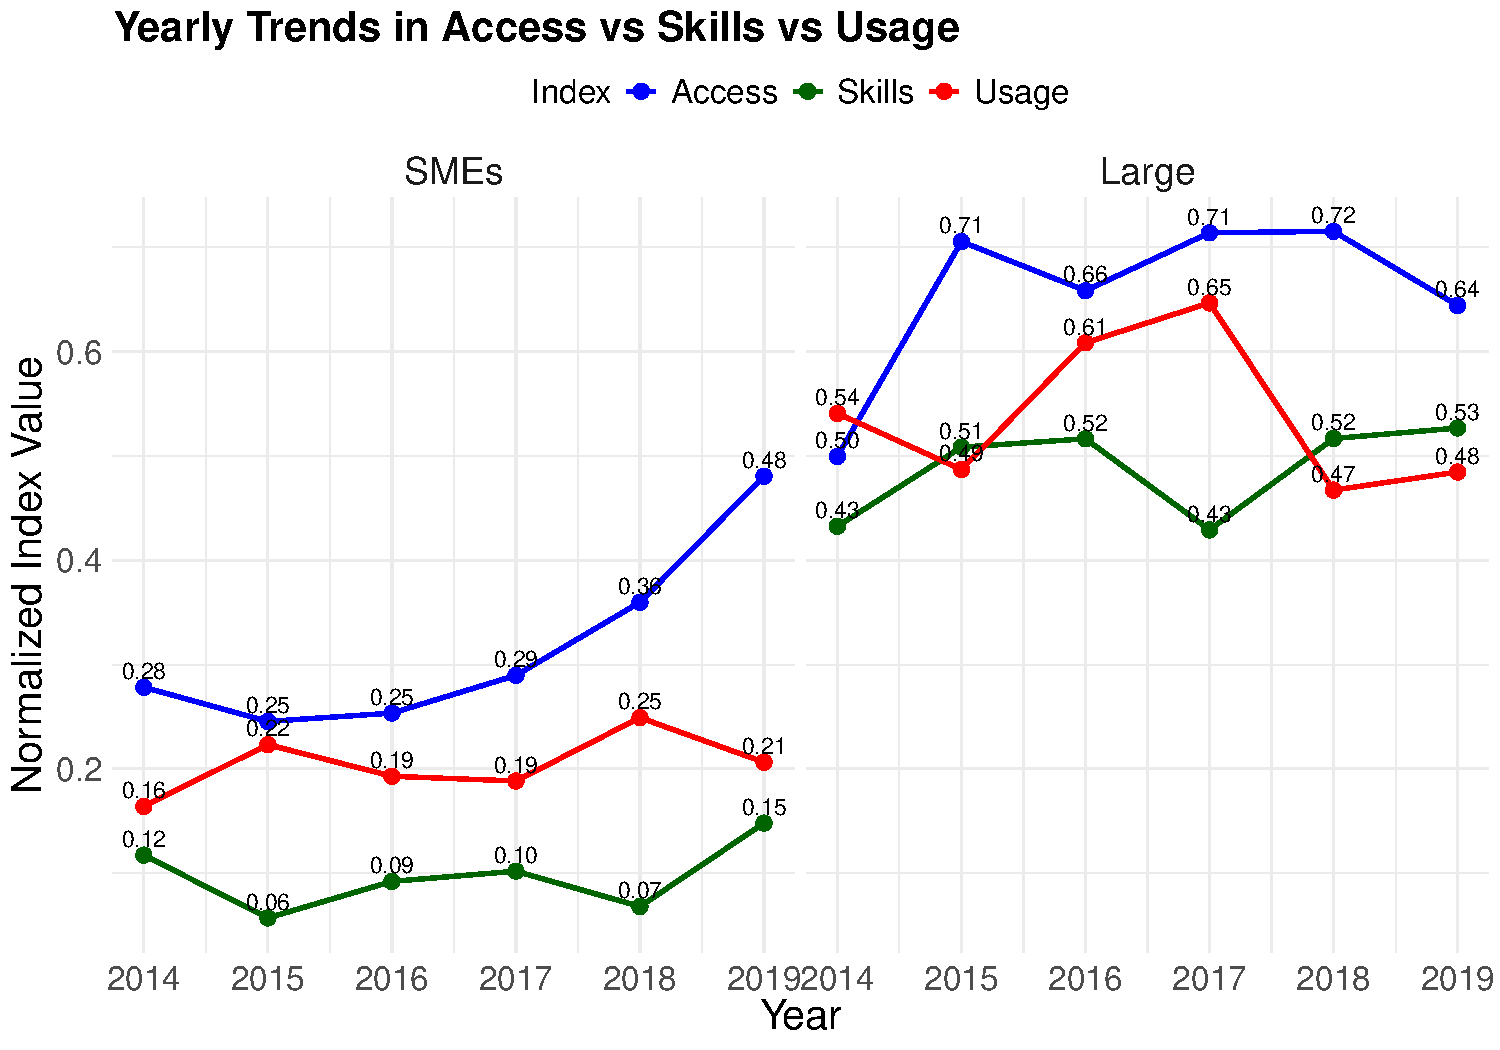
\includegraphics{FactoAnalysisDigitalDivide_files/figure-beamer/yearTrendSize-1.pdf}
\end{frame}

\begin{frame}{7.1. Results II}
\phantomsection\label{results-ii}
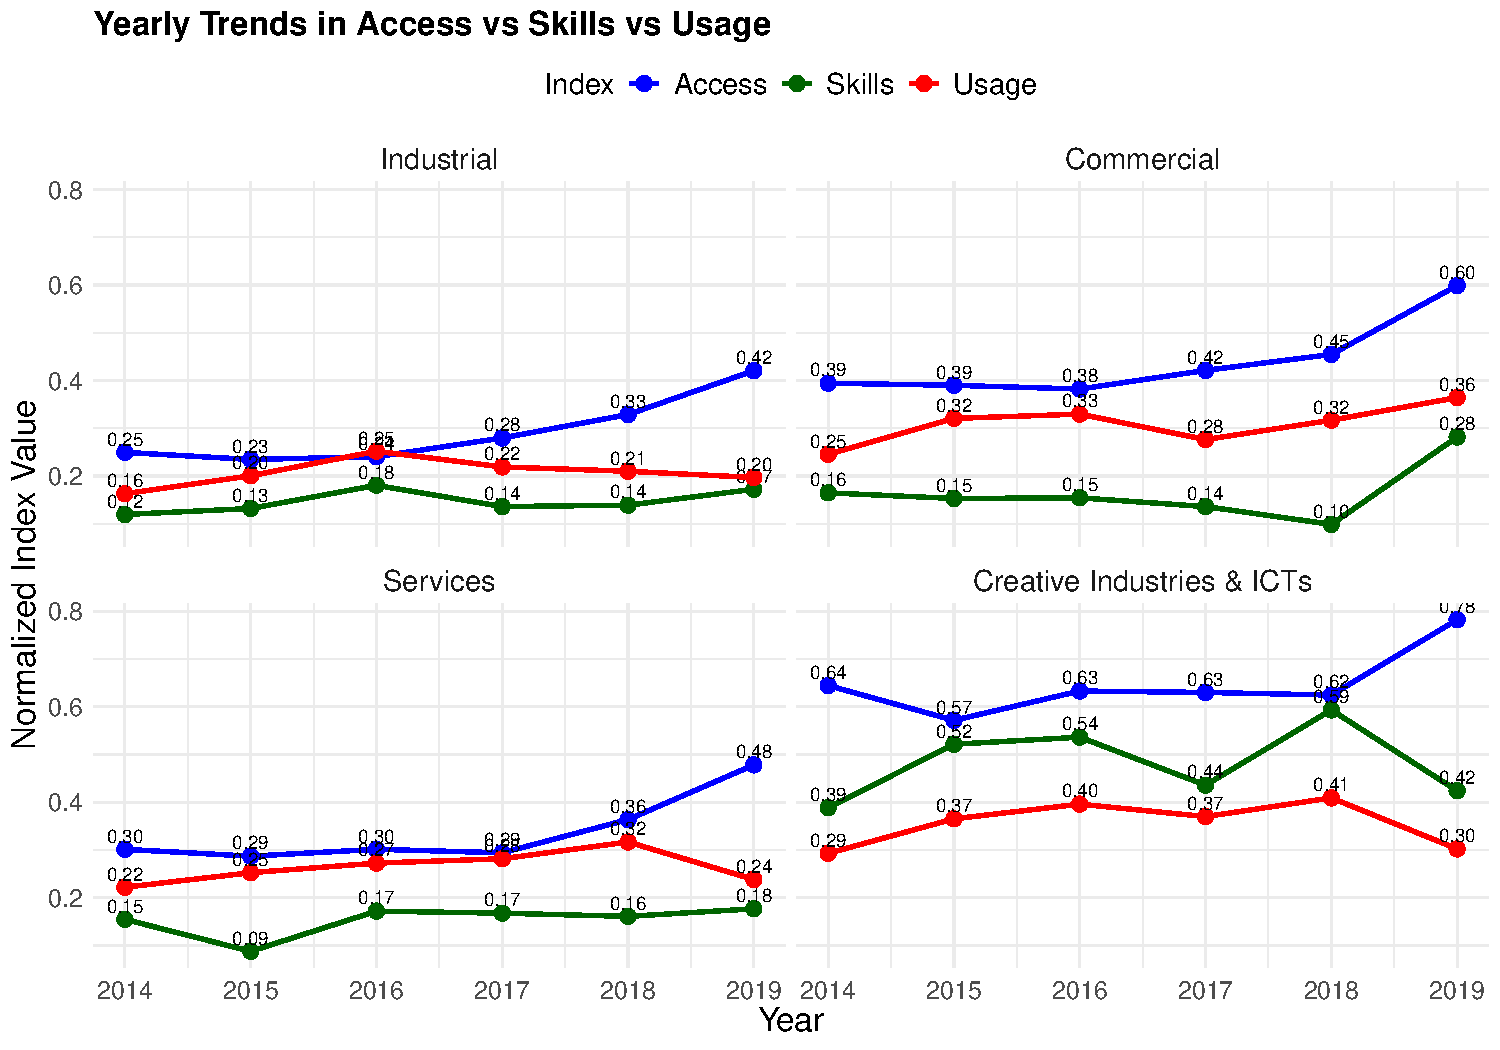
\includegraphics{FactoAnalysisDigitalDivide_files/figure-beamer/yearTrendMac-1.pdf}
\end{frame}

\begin{frame}{7.2. Results III}
\phantomsection\label{results-iii}
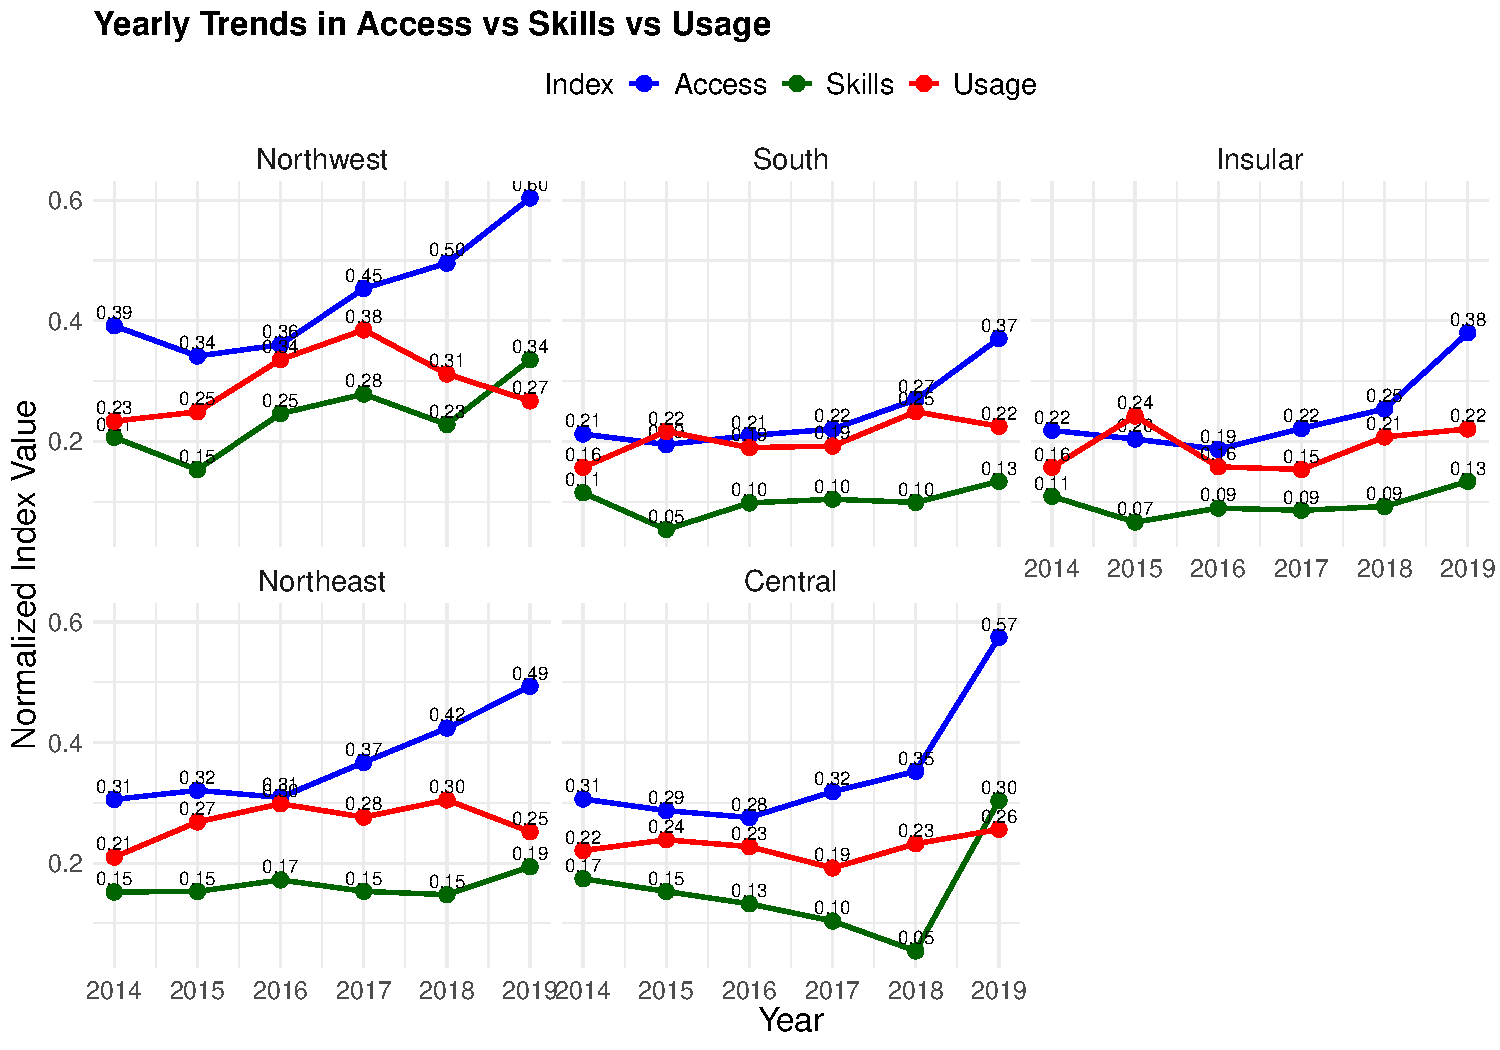
\includegraphics{FactoAnalysisDigitalDivide_files/figure-beamer/yearTrendReg-1.pdf}
\end{frame}

\begin{frame}{8. Q\&A}
\phantomsection\label{qa}
Thank you for your attention
\end{frame}

\renewcommand\refname{References}
\begin{frame}[allowframebreaks]{References}
  \bibliographytrue
  \bibliography{ShiftPatterns.bib}
\end{frame}

\end{document}
